\documentclass{article}
\usepackage{graphicx} % Required for inserting images

\title{ECN 310}
\author{ltsippel }
\date{November 2023}

% set margins and spacing
\addtolength{\textwidth}{1.3in}
\addtolength{\oddsidemargin}{-.65in} %left margin
\addtolength{\evensidemargin}{-.65in}
\setlength{\textheight}{9in}
\setlength{\topmargin}{-.5in}
\setlength{\headheight}{0.0in}
\setlength{\footskip}{.375in}
\renewcommand{\baselinestretch}{1.0}
\linespread{1.0}

% load miscellaneous packages
\usepackage{csquotes}
\usepackage[american]{babel}
\usepackage[usenames,dvipsnames]{color}
\usepackage{graphicx,amsbsy,amssymb, amsmath, amsthm, MnSymbol,bbding,times, verbatim,bm,pifont,pdfsync,setspace,natbib}
\usepackage{float}[H]

% enable hyperlinks and table of contents
\usepackage[pdftex,
bookmarks=true,
bookmarksnumbered=false,
pdfview=fitH,
bookmarksopen=true,hyperfootnotes=false]{hyperref}

% define environments
\newtheorem{definition}{Definition}
\newtheorem{fact}{Fact}
\newtheorem{result}{Result}
\newtheorem{proposition}{Proposition}



\begin{document}
\title{Dementia in the Elderly and Education}
\author{Ixora Artis\and Sophie Haber\and Abigail Mondin\and Luke Sippel}
\date{\vskip-.1in \today}
\maketitle

\vskip.3in
\begin{center} {\bf Abstract} \end{center}
\begin{quote}
{\small This paper aims to answer the question “can a person's amount of education and its quality decrease the chances of having dementia or cognitive problems in older age?” by exploring the link between the likelihood of developing dementia and the level of education received. The variables we use include years of education, forgetfulness during daily activities, has the person ever had dementia, getting lost in familiar places, earning a college degree, and earning a high school diploma/GED. We compiled a variety of charts and graphs to analyze our data and eventually reach our conclusion. Evidence from the literature review established a connection between the amount of education received and the eventual development of dementia. Our literature review also established a preliminary connection between how long you're in school/highest level of education and receiving an eventual dementia diagnosis. Our data set isn't quite thorough enough to establish a concrete connection between dementia and the level and years of higher education—however, some data shows a semblance of a connection between education and the development of dementia.}
\end{quote}

\bigskip
\section{Introduction} \label{sec:introduction}
\hspace*{1em} The relationship between education and dementia has been studied previously from many different angles. In our research, we specifically looked at how the amount of education one receives impacts their chance of developing dementia or other cognitive problems later in life. This is an important relationship for society to understand as a majority of individuals will receive some form of education for a given duration of time, as well as live into their older ages. Knowing how one affects the other can help us take steps to prevent the development of dementia in future generations, but also recognize the likelihood of an individual developing dementia or another cognitive problem. 

This topic was presented to us by Professor Flores-Lagunes, an economics professor at Syracuse University, in a much broader question. For our purposes, we chose to narrow down the question and focus on how the amount of education an individual receives impacts their cognitive health and chance of developing dementia. This topic resonates with each member of our team for various reasons, but ultimately, we all have a general interest in the topic and thought it is critical to better understand the relationship between the two and their possible implications.

Throughout our research we hope to answer the following question: Can a person’s amount of education and its quality decrease the chances of having dementia or cognitive problems in older ages? We will do this by utilizing the 2016 RAND Health and Retirement Study (HRS). This is a study that is utilized by researchers and analysts looking to study aging. It collects health and socioeconomic information from respondents over the age of 50. Initially, when the topic was presented to us, the 2016 Harmonized Cognitive Assessment Protocol (HCAP) was the supporting data set recommended to us. However, this did not contain any information on the respondent’s education, and because of this, we pivoted to use the 2016 RAND HRS data set. There is more current data available than the year 2016, but we chose to stick with this year since the faculty member who recommended the HCAP data had suggested the year 2016. Using the 2016 RAND HRS data, we will look at variables such as forgetfulness or getting lost as an indicator of cognitive health and compare those to the number of years of education the respondents received and whether or not they have dementia. 

Unfortunately, we do not believe that we have found very much definitive proof that long-term education improves cognitive health and reduces the chance of developing dementia. However, in figures throughout our report, there are indicators that our hypothesis is not definitively wrong either. There is still much room for exploration in this field of research. Had we had more time or resources, we would have liked to look at more variables that could be used as indicators of cognitive health, look at the data available for this topic across countries, and consider how economic status may impact education and in turn, dementia. 

In section~\ref{sec:literature}, we review the existing literature. In section~\ref{sec:theory}, we analyze theory in relation to our hypothesis. In section~\ref{sec:data}, we describe our data. In section~\ref{sec:result}, we explain our analysis and illustrate what our results mean. In section~\ref{sec:conclusion}, we conclude and summarize our findings.

\section{Literature Review} \label{sec:literature}

\hspace*{1em} We have chosen to analyze articles that look at the link between years of education, the highest level of education achieved, and dementia. "Does education improve cognitive performance four decades after school completion? This article relates to our research question as it establishes the connection between cognition and higher education levels. Higher Education allows you to get into an industry that requires skilled labor. Skilled Labor allows you to exercise your brain while maintaining a higher level of cognition. Higher education allows you to increase your brain usage in other parts of everyday life, which helps maintain the brain. This connects to our research as it highlights the relationship between education and dementia related to cognition and brain function. Similarly, “The Causal Effect of Education on Earnings" talks about how education opens the door for skilled labor which requires higher brain usage. In addition, it talks about how your level has an impact on your earnings because wealth is a part of the economic development of countries and individuals. "The effect of education on old age cognitive abilities: evidence from a regression discontinuity design" is about how if you are at a higher economic level, you have access to a better-quality education and access to higher education. This lessens the chance that you develop dementia due to schooling. However early education development is more critical, especially among g people from disadvantaged backgrounds. This relates to our research as it highlights the relationship between education and the probability of developing dementia. "A Comparison of the Prevalence of Dementia in the United States in 2000 and 2012" shows that there has been a decrease in the number of people affected by dementia in the last 10 years by 11.6\%. The study attributes this to education as higher education is associated with a lower risk of developing dementia. This relates to our research because we investigate whether or not education impacts the chances of developing dementia. "Compulsory Education and the Benefits of Schooling by Melvin Stephens, Jr. Yang", this article investigates if within homogeneous groups government-required education has an impact on whether or not you develop dementia. This is dis-proven by the article as they argue it has little to no impact. This relates to our research as some of our variable sets include grades 0-12. The literature review highlights the return on education and the connection between the socioeconomic status you achieve to higher education. Education is shown to impact your level of cognition via labor force participation and activities. Education has an impact on earnings which relate to the level of skill you use on a day-to-day basis which contributes to your level of cognition which is a major factor for dementia. Higher levels of education are said to improve your cognition, lowering the probability of developing dementia. There is data available for other countries, such as Europe, but we focused on the United States. Our research answers the question by comparing the level of education and years of people who have developed dementia.Discuss at least five papers that are closely related to your results (more is better). Explain how they're related. Did you find something similar, or different? Did you look at a different context? Different time period? Different level of detail?

\section{Theoretical Analysis} \label{sec:theory}
\hspace*{1em} As Banks and Mazzonna (2012) point out, it is difficult to clearly identify the specific mechanism through which education affects cognitive abilities in older ages. However, to investigate whether prolonged education can reduce the chance of developing dementia or cognitive problems in older ages, we will look at the idea that education is a pathway to better cognitive health. Following the theory of Schneeweis, Skirbekk, and Winter-Ember (2014), we looked at prolonged education as an intellectually stimulating activity that is beneficial for cognitive maintenance, as well as giving individuals the skills and knowledge for other intellectually stimulating activities that support the upkeep of one’s mind. An increase in the amount of education a person receives directly impacts the skills and knowledge they have, which then improves their cognitive health and decreases the chance that an individual will develop dementia or other cognitive problems later in life (see figure~\ref{fig:causal diagram}). If our hypothesis is correct, we would expect to see a relatively negative relationship between the percentage of people who have developed dementia and the number of years of education that they received. This means that if a person received zero, one, two, or three years of education we would expect to see a higher percentage of people who have developed dementia than if a person has received fourteen, fifteen, sixteen, or seventeen years of education. 

\begin{figure}[h!]
    \centering
    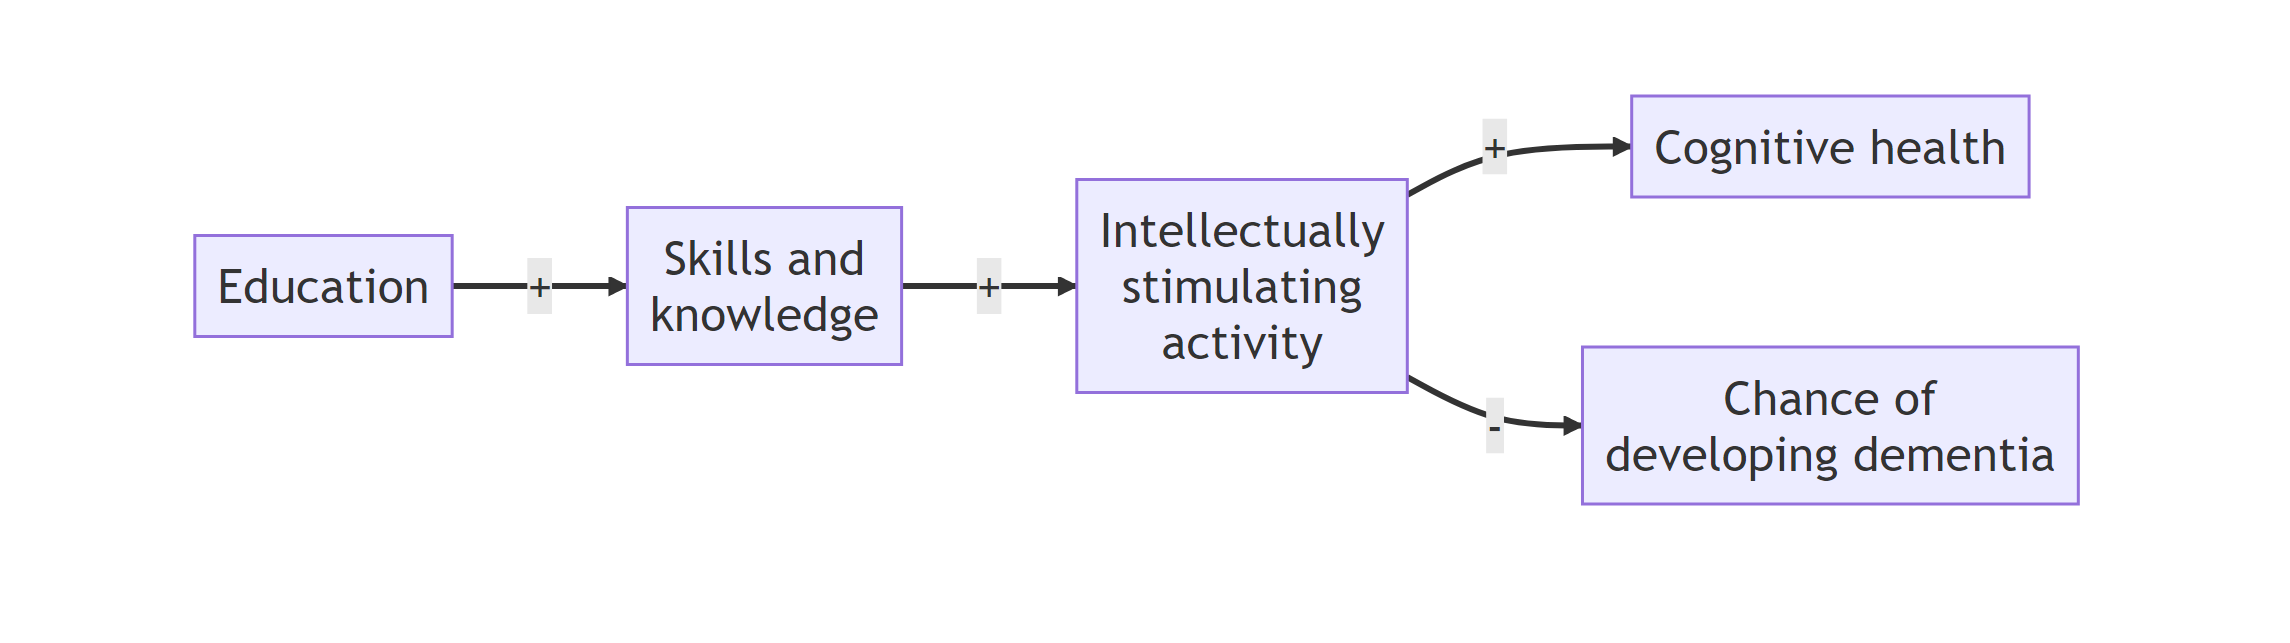
\includegraphics[width=0.8\linewidth]{causal_diagram.png}
    \caption{Causal Diagram}
    \label{fig:causal diagram}
\end{figure}

\section{Data}
\label{sec:data}
\hspace*{1em}The 2016 RAND HRS includes thousands of variables, that we chose to cut down to better understand and investigate the topic at hand. We looked at a breakdown of different education levels, variables that we deemed good measures of cognitive health, and reports of ever having dementia. We compared these variables to produce the following graphs.

\begin{figure}[h!]
    \centering
    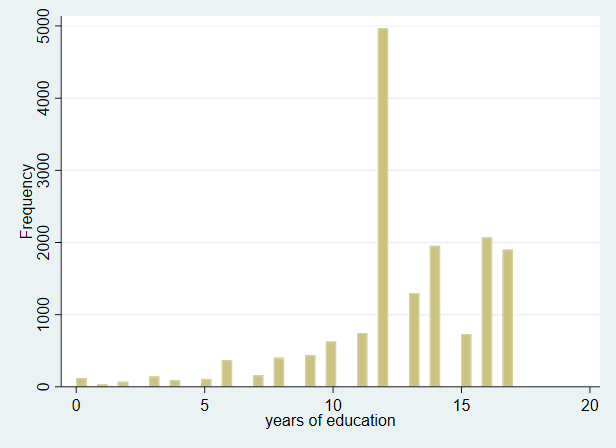
\includegraphics[width=0.5\linewidth]{frequency_histogram_pz216.png}
    \caption{Years of Education Frequency}
    \label{fig:histogram}
\end{figure}

\begin{figure}[H]
    \centering
    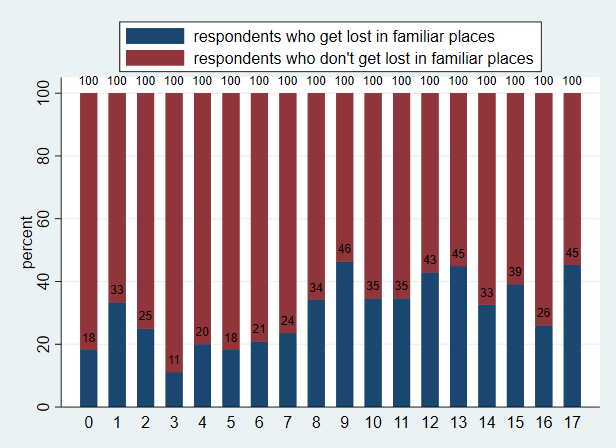
\includegraphics[width=0.5\linewidth]{updated_pd554_over_pz216.png}
    \caption{Getting Lost in Familiar Places Versus Years of Education}
    \label{fig:get lost/education}
\end{figure}

\begin{figure}[h!]
    \centering
    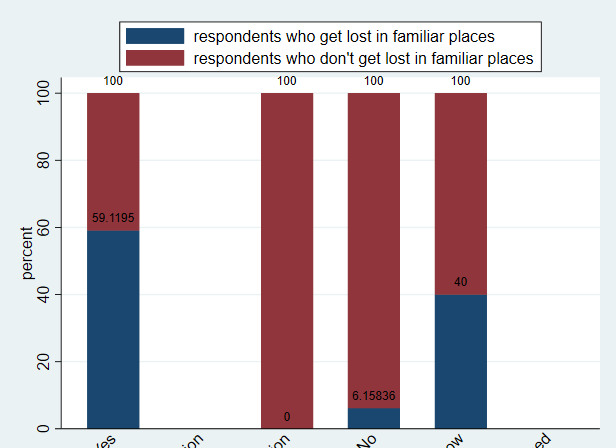
\includegraphics[width=0.5\linewidth]{updated_pd554_over_pc273.png}
    \caption{Getting Lost in Familiar Places Versus Ever Having Dementia}
    \label{fig:get lost/dementia}
\end{figure}

\begin{figure}[h!]
    \centering
    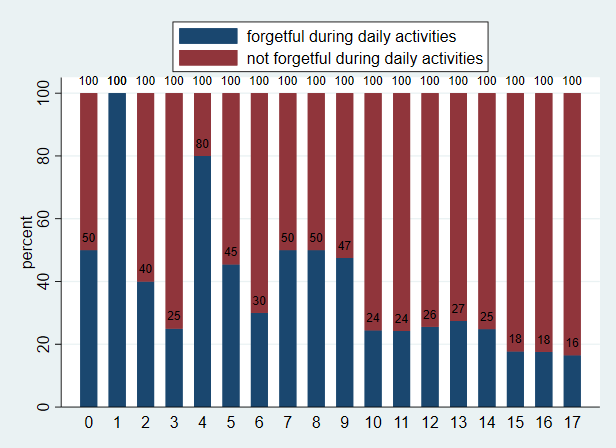
\includegraphics[width=0.5\linewidth]{updated_pv009_over_pz216.png}
    \caption{Forgetful During Daily Activities Versus Years of Education}
    \label{fig:forgetful/education}
\end{figure}

\begin{figure}[h!]
    \centering
    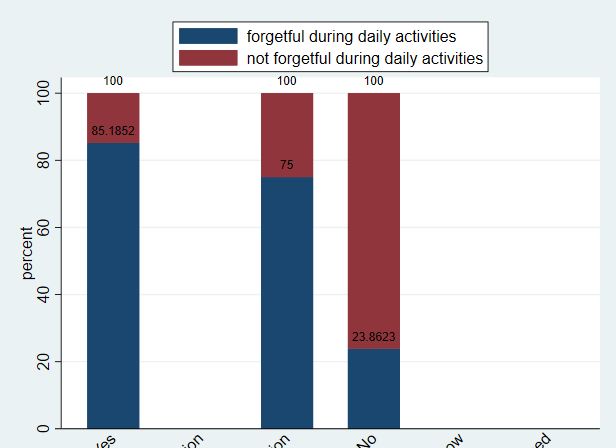
\includegraphics[width=0.5\linewidth]{updated_pv009_over_pc273.png} \caption{Forgetful During Daily Activities Versus Ever Having Dementia}
    \label{fig:forgetful/dementia}
\end{figure}

\begin{figure}[H]
    \centering
    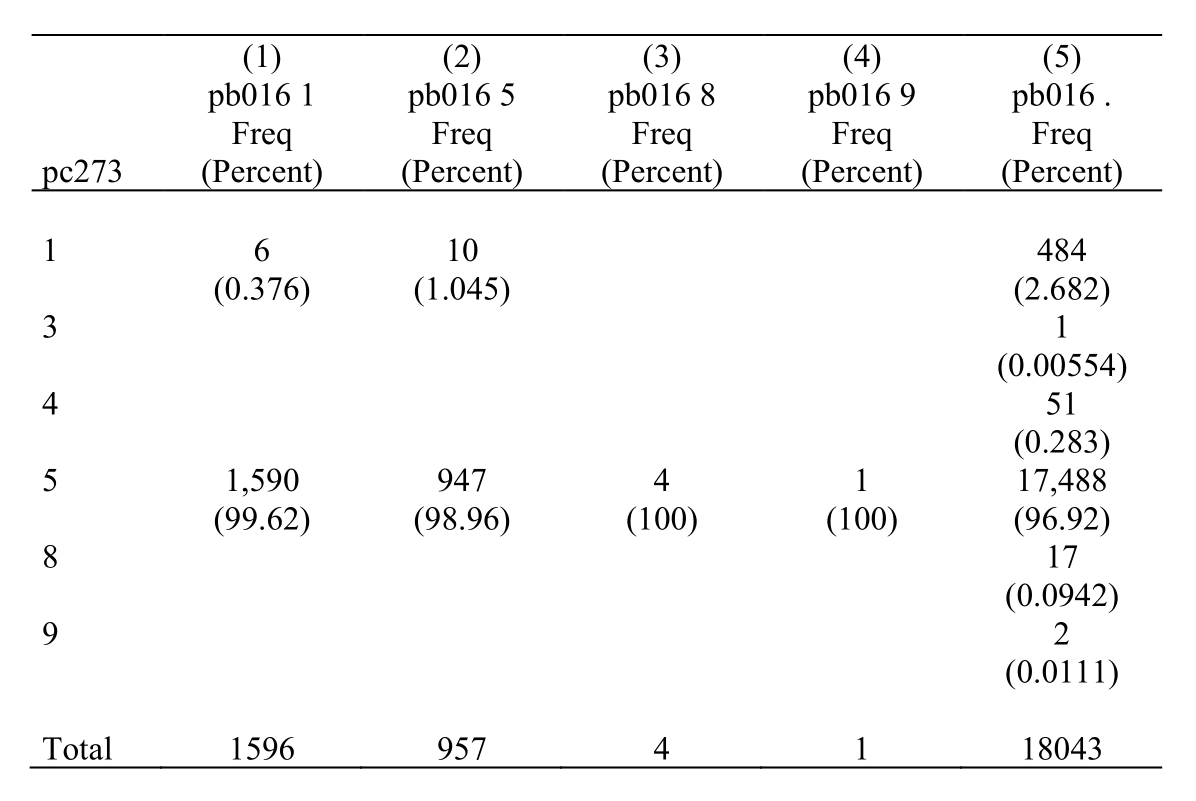
\includegraphics[width=0.75\linewidth]{college degree v dementia.png}
    \caption{College Degree Versus Dementia}
    \label{fig:college/dementia}
\end{figure}

\begin{figure}[H]
    \centering
    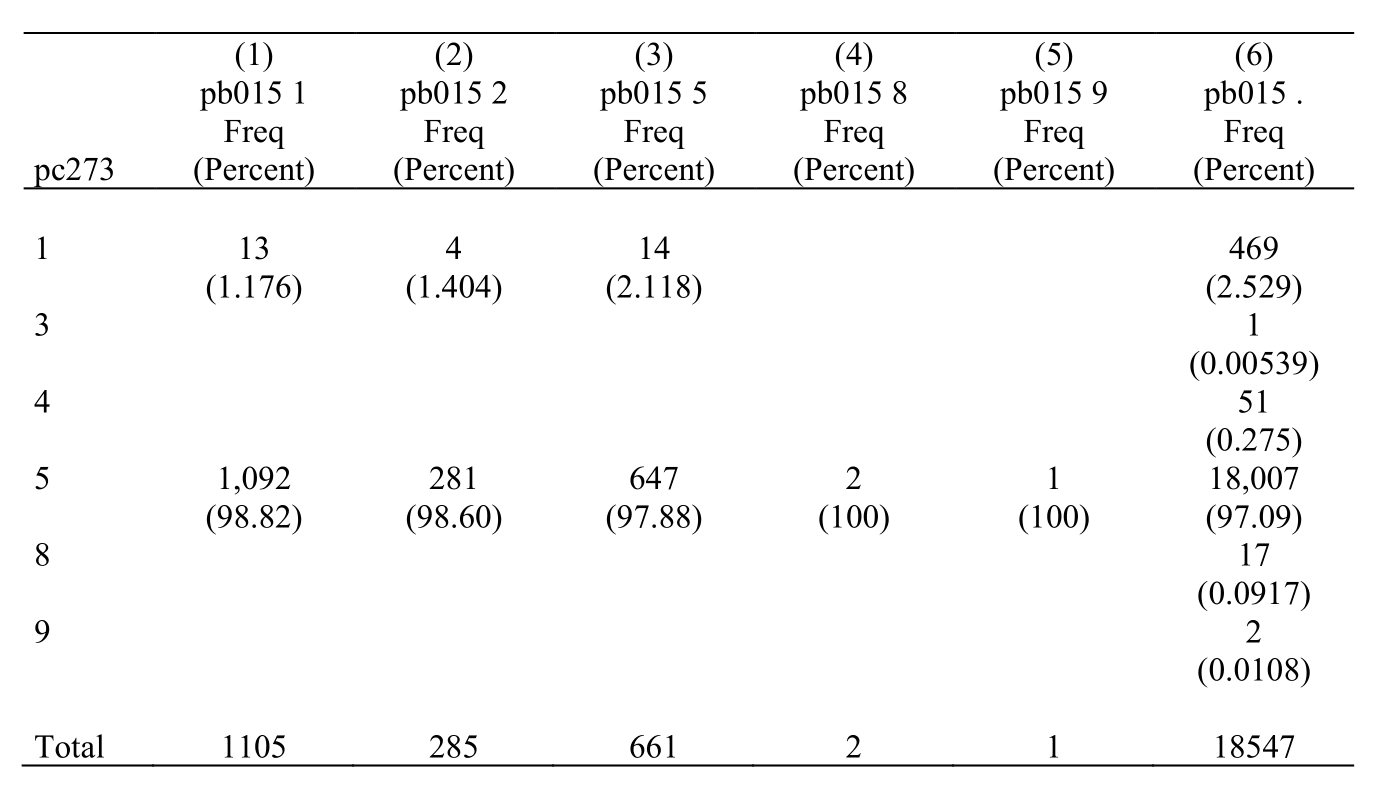
\includegraphics[width=0.75\linewidth]{high school ged v dementia.png}
    \caption{High School + GED Versus Dementia}
    \label{fig:high school/dementia}
\end{figure}

\begin{center}
\begin{tabular}{ |c|c|c| }
    \hline
  & pz216 & pc273 \\ 
  \hline
 pz216 & 1.0000 &  \\  
 \hline
 pc273 & 0.0496
 0.0000 & 1.000 \\
 \hline 
\end{tabular}
\end{center}

 Pwcorr can be used as a connection between the two variables, in our case, having a college degree and having a dementia diagnosis. The p-value is 0.000. Since this is less than 0.05, the correlation between these two variables is statistically significant. The correlation coefficient measurement ranges from -1 to 1, -1 states there is a perfect negative relationship, 0 symbolizes there is no relationship, and 1 demonstrates a perfect positive relationship. Summarize and tab1 provide background for pwcorr and help with the interpretation. 

\section{Analysis and Results}
\label{sec:result}

\hspace*{1em} We used our causal diagram (Figure~\ref{fig:causal diagram}) to frame our variable exploration around our hypothesis, only selecting variables that provide insight into the relationship between reports of dementia diagnosis and educational background as well as the association of this diagnosis with common symptoms. We hypothesized that a higher level of education would lead to a reduced chance of being diagnosed with dementia later on in life.  

\hspace*{1em} In Figure~\ref{fig:college/dementia}, the amount of people who earned their college degree is plotted against reporting dementia diagnosis. We are focusing our analysis on the intersection of row 1 and column 1, row 1 and column 2, row 5 and column 1, and row 5 and column 2. These results were not as telling as we were expecting as 6 people who had a college degree also have dementia compared to the 10 people who denied having dementia and also a college degree. This trend repeats in row 5 with people who do not have dementia, with 947 with no college degree being compared with 1,590 with one. There is not a significant difference between those who have dementia and have or have not earned a college degree even though there are 4 more people without dementia who do have a college degree. The number of people who don’t have dementia but do have a college degree is greater than those who don’t have a college degree without dementia by 643. This shows us some degree of a relationship between the two factors and both results also support our hypothesis. The low numbers also make sense because in college you can specialize your learning to what interests you and comes most naturally. Those who can afford a college education and choose to earn one are consistently using the same areas of their brain to address similar subjects within a specific field. 


\hspace*{1em} In Figure~\ref{fig:high school/dementia}, the table shows the numbers of people who earned their high school diploma or GED against dementia diagnosis. The statistics of interest to us are in the intersection of row 1 and column 1, row 1 and column 2, row 1 and column 3, row 5 and column 1, row 5 and column 2, and row 5 and column 3. Column 2 is reporting those who responded “yes” to earning their GED rather than high school diploma, which can be found in column 1. We saw that there are similar numbers in row 1: 13 people who have dementia and a high school degree, 4 people who have dementia and a GED, and 14 people who have dementia with neither degree. These results are not that helpful in figuring out the validity of our hypothesis because of the closeness of the values, and they are also showing those who have been diagnosed with dementia rather than not. In row 5, which is showing people who have not been diagnosed with dementia, 281 people with a GED have not been diagnosed, along with 1,092 with a high school diploma and 647 without. There is a larger group of people who have a high school diploma and no dementia diagnosis as compared to any of the findings in this table. This aligns with our expectations as high school curricula are quite standardized and everyone receives a similar education that attempts to stimulate the same brain areas in each student. Those who receive a GED normally participate in the program after high school age, which would cause their brains to be less susceptible to growth and strengthening.  

\hspace*{1em} Figure~\ref{fig:histogram}, is a histogram showing the years of education and the frequency of that answer. The large spike at 12 mostly represents senior year of high school, which is normally the last required year of formal education for students in the US. However, the question was quite ambiguous and it is up to the interviewee to define what years of education mean to them and provide an answer based on that. For example, if they were a doctor, they could be defining this through the lens of their specific training for their job rather than lifelong. Figure 3 should have a much larger reported number of people who earned their high school diploma, which also leads us to believe some people who were answering this question might have started their final year of high school but not completed it, which would lead to the difference in numbers that we see. 

\hspace*{1em} The graph of getting lost in familiar places over years of education (Figure~\ref{fig:get lost/education}) shows a weak relationship between those who get lost/don’t get lost and how many years of education they have received. The red bars that correspond with not getting lost in familiar places are longest (highest frequency) towards the lower years of education, rather than the expected higher years of education. This could partially be due to different interpretations of what “years of education” is defining. We see the middle value of years of education (8), starting a trend of 26\% or more of people getting lost in familiar places, which does not support our hypothesis in the big picture. Under the assumption that years of education is directly related to grades (ex. 8 years of education is 8th grade), those who finished middle school and possibly more have more of this dementia symptom experience than those who have anywhere from 1-7 years of education.

\hspace*{1em} In Figure~\ref{fig:get lost/dementia}, which is zooming in on getting lost in familiar places versus reporting a dementia diagnosis, we see the higher frequency of those who responded “yes” to getting lost in familiar places are categorized at 1 on the x-axis (“yes” to having dementia). The reverse happens at 5, which is where the respondent is saying they don’t have dementia, and more people are also reporting they are not getting lost in familiar places. Here, the number of people who deny getting lost in familiar places are extraordinarily higher in people who don’t have dementia than those who do (93.84164\% versus 40.8805\%). However, just like Figure~\ref{fig:get lost/education}, this does not provide a strong indication that our hypothesis is correct, as not getting lost in a familiar place would be a symptom of not having dementia. 

\hspace*{1em} However, looking at forgetfulness during daily activities over years of education provides stronger evidence of a relationship in Figure~\ref{fig:forgetful/education}. There is a clear steady increase in those who responded “no” to being forgetful as their reported years of education increase. At year 10 of education, there is much less staggering in the results and it is consistent in showing a lower level of forgetfulness. This supports our hypothesis by showing that higher years of education correspond with lower incidences of memory loss in daily life. We further inferred that this is due to the brain processes being continually strengthened while in school. 

\hspace*{1em} When forgetful during daily activities was plotted against ever had dementia (Figure~\ref{fig:forgetful/dementia}), we can see that those who responded “yes” to being forgetful during daily activities and also having dementia are the larger spike while at 5 on the x-axis (representing someone who does not have dementia), has the largest spike for not being forgetful. While this makes sense as being forgetful during daily activities is a symptom of dementia, our analysis of the results from Figure~\ref{fig:forgetful/dementia} combined with those from Figure~\ref{fig:forgetful/education} support our hypothesis even more as they indicate that the increase in years of schooling stimulates brain activity which further increases cognitive health.

\hspace*{1em} Our analysis and interpretations of the graphs and tables we created led us to believe our hypothesis and theory were on the right track. While we don't yet have definitive proof of a connection between high levels of education and preventing a dementia diagnosis, we can see a relationship between important cognitive processes that are stimulated by a more thorough education lessening the number of dementia diagnoses. 

\section{Conclusion}
\label{sec:conclusion}

\hspace*{1em} This research shows that more work can still be done to dissect the relationship between education and dementia. While answering “if a person’s amount of education and its quality decrease the chances of having dementia or cognitive problems in older ages” we have not concluded enough definitive analysis to strongly support our hypothesis. However, some of our data was indicative of a prolonged education decreasing the likelihood of dementia. 

In review, we took the 2016 RAND Health and Retirement Study(HRS) code book to extract useful variables. Variables like years of education and getting lost in familiar places did not express a definitive conclusion because some of the results aligned with respondents who had shorter years of education, rather than what we were expecting. Yet, it is evident that the analysis of other variables indeed supports our hypothesis. Interpretation of ‘forgetful during daily activities’ compared to both ‘ever having dementia’ and ‘years of education’ both positively impact the formation of our hypothesis. A clear increase was shown between the amount of education and not being forgetful during daily activities. Likewise, in Figure ~\ref{fig:forgetful/dementia} the respondent indicated “yes” to being forgetful during daily activities and having dementia and “no” to being forgetful during daily activities and having dementia. Ultimately, we made the inference that the more time respondents spent in school the less likely they were to develop and or have dementia. 

The question becomes what can we do with this inference? We have not found definitive proof that long-term education improves cognitive health and reduces the chance of developing dementia. Yet, we have found that the longer respondents stayed in school the less forgetful during daily activities they were likely to be, even earning a high school diploma or GED has lowered the frequency of dementia diagnosis. More research can come from this on a broader scale, including more indicators of cognitive health from a larger sample size, including more countries. Another possible variable of interest could also be continued education in older ages.

\newpage
\section*{Bibliography}
\singlespacing 
\hspace*{1em} 1  Schneeweis, Nicole, Vegard Skirbekk, and Rudolf Winter-Ebmer. "Does education improve cognitive performance four decades after school completion?." Demography 51, no. 2 (2014): 619-643. Available at https://read.dukeupress.edu/demography/article/51/2/619/169438/Does-Education-Improve-Cognitive-Performance-Four.

2  Banks, James, and Fabrizio Mazzonna. "The effect of education on old age cognitive abilities: evidence from a regression discontinuity design." The Economic Journal 122, no.
560 (2012): 418-448.

https://academic.oup.com/ej/article/122/560/418/5079978


3 Card, D. (1999), “The Causal Effect of Education on Earnings,” in Handbook of Labor Economics 
     (Vol. 3A), eds. O. Ashenfelter and D. Card, Amsterdam: North Holland, pp. 1801–1863 

https://davidcard.berkeley.edu/papers/causaleducearnings.pdf


4  Stephens, Melvin, and Dou-Yan Yang. Compulsory education and the benefits of schooling, 2013. https://doi.org/10.3386/w19369.


5  Langa, Kenneth M., Eric B. Larson, Eileen M. Crimmins, Jessica D. Faul, Deborah A. Levine, Mohammed U. Kabeto, and David R. Weir. “A Comparison of the Prevalence of Dementia in the United States in 2000 and 2012.” JAMA Internal Medicine 177, no. 1 (2017): 51. https://doi.org/10.1001/jamainternmed.2016.6807.
\setlength\bibsep{10pt}

\end{document}


